% Options for packages loaded elsewhere
\PassOptionsToPackage{unicode}{hyperref}
\PassOptionsToPackage{hyphens}{url}
%
\documentclass[
]{article}
\usepackage{lmodern}
\usepackage{amssymb,amsmath}
\usepackage{ifxetex,ifluatex}
\ifnum 0\ifxetex 1\fi\ifluatex 1\fi=0 % if pdftex
  \usepackage[T1]{fontenc}
  \usepackage[utf8]{inputenc}
  \usepackage{textcomp} % provide euro and other symbols
\else % if luatex or xetex
  \usepackage{unicode-math}
  \defaultfontfeatures{Scale=MatchLowercase}
  \defaultfontfeatures[\rmfamily]{Ligatures=TeX,Scale=1}
\fi
% Use upquote if available, for straight quotes in verbatim environments
\IfFileExists{upquote.sty}{\usepackage{upquote}}{}
\IfFileExists{microtype.sty}{% use microtype if available
  \usepackage[]{microtype}
  \UseMicrotypeSet[protrusion]{basicmath} % disable protrusion for tt fonts
}{}
\makeatletter
\@ifundefined{KOMAClassName}{% if non-KOMA class
  \IfFileExists{parskip.sty}{%
    \usepackage{parskip}
  }{% else
    \setlength{\parindent}{0pt}
    \setlength{\parskip}{6pt plus 2pt minus 1pt}}
}{% if KOMA class
  \KOMAoptions{parskip=half}}
\makeatother
\usepackage{xcolor}
\IfFileExists{xurl.sty}{\usepackage{xurl}}{} % add URL line breaks if available
\IfFileExists{bookmark.sty}{\usepackage{bookmark}}{\usepackage{hyperref}}
\hypersetup{
  pdftitle={Results of PangoVis},
  pdfauthor={Devan Becker},
  hidelinks,
  pdfcreator={LaTeX via pandoc}}
\urlstyle{same} % disable monospaced font for URLs
\usepackage[margin=1in]{geometry}
\usepackage{color}
\usepackage{fancyvrb}
\newcommand{\VerbBar}{|}
\newcommand{\VERB}{\Verb[commandchars=\\\{\}]}
\DefineVerbatimEnvironment{Highlighting}{Verbatim}{commandchars=\\\{\}}
% Add ',fontsize=\small' for more characters per line
\usepackage{framed}
\definecolor{shadecolor}{RGB}{248,248,248}
\newenvironment{Shaded}{\begin{snugshade}}{\end{snugshade}}
\newcommand{\AlertTok}[1]{\textcolor[rgb]{0.94,0.16,0.16}{#1}}
\newcommand{\AnnotationTok}[1]{\textcolor[rgb]{0.56,0.35,0.01}{\textbf{\textit{#1}}}}
\newcommand{\AttributeTok}[1]{\textcolor[rgb]{0.77,0.63,0.00}{#1}}
\newcommand{\BaseNTok}[1]{\textcolor[rgb]{0.00,0.00,0.81}{#1}}
\newcommand{\BuiltInTok}[1]{#1}
\newcommand{\CharTok}[1]{\textcolor[rgb]{0.31,0.60,0.02}{#1}}
\newcommand{\CommentTok}[1]{\textcolor[rgb]{0.56,0.35,0.01}{\textit{#1}}}
\newcommand{\CommentVarTok}[1]{\textcolor[rgb]{0.56,0.35,0.01}{\textbf{\textit{#1}}}}
\newcommand{\ConstantTok}[1]{\textcolor[rgb]{0.00,0.00,0.00}{#1}}
\newcommand{\ControlFlowTok}[1]{\textcolor[rgb]{0.13,0.29,0.53}{\textbf{#1}}}
\newcommand{\DataTypeTok}[1]{\textcolor[rgb]{0.13,0.29,0.53}{#1}}
\newcommand{\DecValTok}[1]{\textcolor[rgb]{0.00,0.00,0.81}{#1}}
\newcommand{\DocumentationTok}[1]{\textcolor[rgb]{0.56,0.35,0.01}{\textbf{\textit{#1}}}}
\newcommand{\ErrorTok}[1]{\textcolor[rgb]{0.64,0.00,0.00}{\textbf{#1}}}
\newcommand{\ExtensionTok}[1]{#1}
\newcommand{\FloatTok}[1]{\textcolor[rgb]{0.00,0.00,0.81}{#1}}
\newcommand{\FunctionTok}[1]{\textcolor[rgb]{0.00,0.00,0.00}{#1}}
\newcommand{\ImportTok}[1]{#1}
\newcommand{\InformationTok}[1]{\textcolor[rgb]{0.56,0.35,0.01}{\textbf{\textit{#1}}}}
\newcommand{\KeywordTok}[1]{\textcolor[rgb]{0.13,0.29,0.53}{\textbf{#1}}}
\newcommand{\NormalTok}[1]{#1}
\newcommand{\OperatorTok}[1]{\textcolor[rgb]{0.81,0.36,0.00}{\textbf{#1}}}
\newcommand{\OtherTok}[1]{\textcolor[rgb]{0.56,0.35,0.01}{#1}}
\newcommand{\PreprocessorTok}[1]{\textcolor[rgb]{0.56,0.35,0.01}{\textit{#1}}}
\newcommand{\RegionMarkerTok}[1]{#1}
\newcommand{\SpecialCharTok}[1]{\textcolor[rgb]{0.00,0.00,0.00}{#1}}
\newcommand{\SpecialStringTok}[1]{\textcolor[rgb]{0.31,0.60,0.02}{#1}}
\newcommand{\StringTok}[1]{\textcolor[rgb]{0.31,0.60,0.02}{#1}}
\newcommand{\VariableTok}[1]{\textcolor[rgb]{0.00,0.00,0.00}{#1}}
\newcommand{\VerbatimStringTok}[1]{\textcolor[rgb]{0.31,0.60,0.02}{#1}}
\newcommand{\WarningTok}[1]{\textcolor[rgb]{0.56,0.35,0.01}{\textbf{\textit{#1}}}}
\usepackage{graphicx}
\makeatletter
\def\maxwidth{\ifdim\Gin@nat@width>\linewidth\linewidth\else\Gin@nat@width\fi}
\def\maxheight{\ifdim\Gin@nat@height>\textheight\textheight\else\Gin@nat@height\fi}
\makeatother
% Scale images if necessary, so that they will not overflow the page
% margins by default, and it is still possible to overwrite the defaults
% using explicit options in \includegraphics[width, height, ...]{}
\setkeys{Gin}{width=\maxwidth,height=\maxheight,keepaspectratio}
% Set default figure placement to htbp
\makeatletter
\def\fps@figure{htbp}
\makeatother
\setlength{\emergencystretch}{3em} % prevent overfull lines
\providecommand{\tightlist}{%
  \setlength{\itemsep}{0pt}\setlength{\parskip}{0pt}}
\setcounter{secnumdepth}{-\maxdimen} % remove section numbering
\usepackage[]{natbib}
\bibliographystyle{plainnat}

\title{Results of PangoVis}
\author{Devan Becker}
\date{2021-04-09}

\begin{document}
\maketitle

\hypertarget{load-packages-and-data}{%
\section{Load Packages and Data}\label{load-packages-and-data}}

\begin{Shaded}
\begin{Highlighting}[]
\CommentTok{\# Packages that Art hates}
\KeywordTok{library}\NormalTok{(dplyr)}
\KeywordTok{library}\NormalTok{(tidyr)}
\KeywordTok{library}\NormalTok{(ggplot2)}
\KeywordTok{library}\NormalTok{(stringr)}
\KeywordTok{library}\NormalTok{(here)}

\NormalTok{dirich \textless{}{-}}\StringTok{ }\OtherTok{TRUE} \CommentTok{\#params$dirich}

\CommentTok{\# Read in CSV files}
\NormalTok{csvs \textless{}{-}}\StringTok{ }\KeywordTok{list.files}\NormalTok{(}\KeywordTok{here}\NormalTok{(}\StringTok{"data/"}\NormalTok{, }\StringTok{"pangolineages"}\NormalTok{),}
    \DataTypeTok{pattern =} \KeywordTok{ifelse}\NormalTok{(dirich, }\StringTok{"*\_d.csv"}\NormalTok{, }\StringTok{"*.csv"}\NormalTok{),}
    \DataTypeTok{full.names =} \OtherTok{TRUE}\NormalTok{)}

\CommentTok{\# Remove any copies}
\NormalTok{csvs \textless{}{-}}\StringTok{ }\NormalTok{csvs[}\OperatorTok{!}\KeywordTok{grepl}\NormalTok{(}\StringTok{"{-}1"}\NormalTok{, csvs)]}

\CommentTok{\# Bring them into one data frame}
\NormalTok{lins \textless{}{-}}\StringTok{ }\KeywordTok{bind\_rows}\NormalTok{(}\KeywordTok{lapply}\NormalTok{(csvs, read.csv))}

\CommentTok{\# Taxon is encoded as \_ACCSESSIONNUMBER.ID, split into ACCESSIONNUMBER and ID}
\NormalTok{lins \textless{}{-}}\StringTok{ }\NormalTok{lins }\OperatorTok{\%\textgreater{}\%}
\StringTok{    }\KeywordTok{separate}\NormalTok{(}\DataTypeTok{col =} \StringTok{"taxon"}\NormalTok{, }\DataTypeTok{sep =} \StringTok{"}\CharTok{\textbackslash{}\textbackslash{}}\StringTok{."}\NormalTok{,}
        \DataTypeTok{into =} \KeywordTok{c}\NormalTok{(}\StringTok{"taxon"}\NormalTok{, }\StringTok{"sample"}\NormalTok{)) }\OperatorTok{\%\textgreater{}\%}
\StringTok{    }\KeywordTok{mutate}\NormalTok{(}\DataTypeTok{taxon =} \KeywordTok{str\_replace}\NormalTok{(taxon, }\StringTok{"}\CharTok{\textbackslash{}\textbackslash{}}\StringTok{\_"}\NormalTok{, }\StringTok{""}\NormalTok{))}

\NormalTok{badlins \textless{}{-}}\StringTok{ }\KeywordTok{table}\NormalTok{(lins}\OperatorTok{$}\NormalTok{taxon)}
\NormalTok{badlins \textless{}{-}}\StringTok{ }\KeywordTok{names}\NormalTok{(badlins[}\KeywordTok{which}\NormalTok{(badlins }\OperatorTok{\textless{}}\StringTok{ }\DecValTok{1000}\NormalTok{)])}
\KeywordTok{cat}\NormalTok{(}\KeywordTok{length}\NormalTok{(badlins), }\StringTok{" runs were removed for having too few samples."}\NormalTok{)}
\end{Highlighting}
\end{Shaded}

\begin{verbatim}
## 11  runs were removed for having too few samples.
\end{verbatim}

\begin{Shaded}
\begin{Highlighting}[]
\NormalTok{lins \textless{}{-}}\StringTok{ }\KeywordTok{filter}\NormalTok{(lins, }\OperatorTok{!}\NormalTok{taxon }\OperatorTok{\%in\%}\StringTok{ }\NormalTok{badlins)}

\CommentTok{\#\#\#\# Visualize the uncertainty in the base calls {-}{-}{-}{-}}
\NormalTok{taxons \textless{}{-}}\StringTok{ }\KeywordTok{unique}\NormalTok{(lins}\OperatorTok{$}\NormalTok{taxon)}
\KeywordTok{length}\NormalTok{(taxons)}
\end{Highlighting}
\end{Shaded}

\begin{verbatim}
## [1] 82
\end{verbatim}

\hypertarget{abstract-info}{%
\section{Abstract Info}\label{abstract-info}}

\begin{Shaded}
\begin{Highlighting}[]
\NormalTok{summs \textless{}{-}}\StringTok{ }\NormalTok{lins }\OperatorTok{\%\textgreater{}\%}
\StringTok{    }\KeywordTok{group\_by}\NormalTok{(taxon) }\OperatorTok{\%\textgreater{}\%}
\StringTok{    }\KeywordTok{summarise}\NormalTok{(}
        \DataTypeTok{maxperc =} \KeywordTok{mean}\NormalTok{(lineage }\OperatorTok{==}\StringTok{ }\KeywordTok{names}\NormalTok{(}\KeywordTok{sort}\NormalTok{(}\KeywordTok{table}\NormalTok{(lineage),}
            \DataTypeTok{decreasing =} \OtherTok{TRUE}\NormalTok{)[}\DecValTok{1}\NormalTok{]),}
        \DataTypeTok{uniques =} \KeywordTok{length}\NormalTok{(}\KeywordTok{unique}\NormalTok{(lineage)),}
        \DataTypeTok{minpango =} \KeywordTok{min}\NormalTok{(probability),}
        \DataTypeTok{maxpango =} \KeywordTok{max}\NormalTok{(probability),}
        \DataTypeTok{menpango =} \KeywordTok{mean}\NormalTok{(probability),}
        \DataTypeTok{max =} \KeywordTok{names}\NormalTok{(}\KeywordTok{sort}\NormalTok{(}\KeywordTok{table}\NormalTok{(lineage), }\DataTypeTok{decreasing =} \OtherTok{TRUE}\NormalTok{))[}\DecValTok{1}\NormalTok{]))}
\end{Highlighting}
\end{Shaded}

\begin{verbatim}
## `summarise()` ungrouping output (override with `.groups` argument)
\end{verbatim}

\begin{Shaded}
\begin{Highlighting}[]
\KeywordTok{print}\NormalTok{(}\StringTok{"summary info"}\NormalTok{)}
\end{Highlighting}
\end{Shaded}

\begin{verbatim}
## [1] "summary info"
\end{verbatim}

\begin{Shaded}
\begin{Highlighting}[]
\KeywordTok{print}\NormalTok{(summs)}
\end{Highlighting}
\end{Shaded}

\begin{verbatim}
## # A tibble: 82 x 2
##    taxon      maxperc
##    <chr>        <dbl>
##  1 ERR4363387   0.938
##  2 ERR4364007   0.871
##  3 ERR4664555   0.945
##  4 ERR4667618   0.990
##  5 ERR4692364   0.914
##  6 ERR4693034   0.847
##  7 ERR4693061   0.941
##  8 ERR4693079   0.866
##  9 ERR4693537   0.972
## 10 ERR4693605   0.970
## # ... with 72 more rows
\end{verbatim}

\begin{Shaded}
\begin{Highlighting}[]
\DecValTok{1} \OperatorTok{{-}}\StringTok{ }\KeywordTok{mean}\NormalTok{(summs}\OperatorTok{$}\NormalTok{maxperc); }\DecValTok{1} \OperatorTok{{-}}\StringTok{ }\KeywordTok{mean}\NormalTok{(summs}\OperatorTok{$}\NormalTok{menpango)}
\end{Highlighting}
\end{Shaded}

\begin{verbatim}
## [1] 0.09124434
\end{verbatim}

\begin{verbatim}
## Warning: Unknown or uninitialised column: `menpango`.
\end{verbatim}

\begin{verbatim}
## Warning in mean.default(summs$menpango): argument is not numeric or logical:
## returning NA
\end{verbatim}

\begin{verbatim}
## [1] NA
\end{verbatim}

\hypertarget{stacked-bar-plots}{%
\section{Stacked Bar Plots}\label{stacked-bar-plots}}

\begin{Shaded}
\begin{Highlighting}[]
\NormalTok{max\_label \textless{}{-}}\StringTok{ }\KeywordTok{max}\NormalTok{(}\KeywordTok{table}\NormalTok{(lins}\OperatorTok{$}\NormalTok{taxon)) }\OperatorTok{/}\StringTok{ }\DecValTok{40}

\KeywordTok{par}\NormalTok{(}\DataTypeTok{mfrow =} \KeywordTok{c}\NormalTok{(}\DecValTok{15}\NormalTok{, }\DecValTok{1}\NormalTok{), }\DataTypeTok{mar =} \KeywordTok{c}\NormalTok{(}\DecValTok{1}\NormalTok{, }\FloatTok{0.5}\NormalTok{, }\FloatTok{1.5}\NormalTok{, }\FloatTok{0.5}\NormalTok{))}
\ControlFlowTok{for}\NormalTok{ (i }\ControlFlowTok{in} \DecValTok{1}\OperatorTok{:}\DecValTok{38}\NormalTok{) \{}
\NormalTok{    pang \textless{}{-}}\StringTok{ }\NormalTok{lins[lins}\OperatorTok{$}\NormalTok{taxon }\OperatorTok{==}\StringTok{ }\NormalTok{taxons[i], ]}
\NormalTok{    called \textless{}{-}}\StringTok{ }\NormalTok{pang}\OperatorTok{$}\NormalTok{lineage[pang}\OperatorTok{$}\NormalTok{sample }\OperatorTok{==}\StringTok{ }\DecValTok{0}\NormalTok{][}\DecValTok{1}\NormalTok{]}
\NormalTok{    pangtab \textless{}{-}}\StringTok{ }\KeywordTok{sort}\NormalTok{(}\KeywordTok{table}\NormalTok{(pang}\OperatorTok{$}\NormalTok{lineage), }\DataTypeTok{decreasing =} \OtherTok{TRUE}\NormalTok{)}

\NormalTok{    colvec \textless{}{-}}\StringTok{ }\KeywordTok{rep}\NormalTok{(}\StringTok{"grey"}\NormalTok{, }\KeywordTok{length}\NormalTok{(pangtab))}
\NormalTok{    colvec[}\KeywordTok{which}\NormalTok{(}\KeywordTok{names}\NormalTok{(pangtab) }\OperatorTok{==}\StringTok{ }\NormalTok{called)] \textless{}{-}}\StringTok{ "red"}

\NormalTok{    n \textless{}{-}}\StringTok{ }\KeywordTok{sum}\NormalTok{(pangtab }\OperatorTok{\textgreater{}}\StringTok{ }\NormalTok{max\_label)}
    \ControlFlowTok{if}\NormalTok{ (n }\OperatorTok{\textgreater{}}\StringTok{ }\DecValTok{1}\NormalTok{) \{}
\NormalTok{        barlabx \textless{}{-}}\StringTok{ }\KeywordTok{c}\NormalTok{(}\DecValTok{0}\NormalTok{, }\KeywordTok{cumsum}\NormalTok{(pangtab[}\DecValTok{1}\OperatorTok{:}\NormalTok{(n }\OperatorTok{{-}}\StringTok{ }\DecValTok{1}\NormalTok{)])) }\OperatorTok{+}
\StringTok{            }\NormalTok{pangtab[}\DecValTok{1}\OperatorTok{:}\NormalTok{n] }\OperatorTok{/}\StringTok{ }\DecValTok{2}

        \KeywordTok{barplot}\NormalTok{(}\KeywordTok{as.matrix}\NormalTok{(pangtab),}
            \DataTypeTok{col =}\NormalTok{ colvec, }\DataTypeTok{hori =} \OtherTok{TRUE}\NormalTok{, }\DataTypeTok{axes =} \OtherTok{FALSE}\NormalTok{)}
        \KeywordTok{text}\NormalTok{(barlabx, }\FloatTok{0.7}\NormalTok{, }\KeywordTok{names}\NormalTok{(pangtab)[}\DecValTok{1}\OperatorTok{:}\NormalTok{n])}
        \KeywordTok{mtext}\NormalTok{(}\DataTypeTok{side =} \DecValTok{3}\NormalTok{, }\DataTypeTok{text =}\NormalTok{ taxons[i], }\DataTypeTok{cex =} \FloatTok{0.75}\NormalTok{, }\DataTypeTok{las =} \DecValTok{1}\NormalTok{)}
\NormalTok{        pretty\_labels \textless{}{-}}\StringTok{ }\KeywordTok{seq}\NormalTok{(}\DecValTok{0}\NormalTok{, }\KeywordTok{sum}\NormalTok{(pangtab),}
                \DataTypeTok{by =} \KeywordTok{ifelse}\NormalTok{(}\KeywordTok{sum}\NormalTok{(pangtab) }\OperatorTok{\textless{}}\StringTok{ }\DecValTok{2000}\NormalTok{, }\DecValTok{100}\NormalTok{, }\DecValTok{1000}\NormalTok{))}
        \KeywordTok{mtext}\NormalTok{(}\DataTypeTok{side =} \DecValTok{1}\NormalTok{,}
            \DataTypeTok{at =}\NormalTok{ pretty\_labels,}
            \DataTypeTok{text =}\NormalTok{ pretty\_labels,}
            \DataTypeTok{line =} \DecValTok{0}\NormalTok{,}
            \DataTypeTok{cex =} \FloatTok{0.75}
\NormalTok{        )}
\NormalTok{    \} }\ControlFlowTok{else}\NormalTok{ \{}
        \KeywordTok{cat}\NormalTok{(}\StringTok{"Taxon"}\NormalTok{, taxons[i], }\StringTok{"had"}\NormalTok{, }\KeywordTok{length}\NormalTok{(pangtab),}
            \StringTok{"unique calls, with largest accounting for"}\NormalTok{,}
\NormalTok{            pangtab[}\DecValTok{1}\NormalTok{], }\StringTok{"lineage calls, }\CharTok{\textbackslash{}n\textbackslash{}t}\StringTok{ with second place"}\NormalTok{,}
\NormalTok{            pangtab[}\DecValTok{2}\NormalTok{], }\StringTok{". First place was"}\NormalTok{,}
            \KeywordTok{ifelse}\NormalTok{(}\KeywordTok{names}\NormalTok{(pangtab)[}\DecValTok{1}\NormalTok{] }\OperatorTok{==}\StringTok{ }\NormalTok{called, }\StringTok{""}\NormalTok{, }\StringTok{"not"}\NormalTok{),}
            \StringTok{"the conseq call.}\CharTok{\textbackslash{}n}\StringTok{"}\NormalTok{)}
\NormalTok{    \}}
\NormalTok{\}}
\end{Highlighting}
\end{Shaded}

\begin{verbatim}
## Taxon ERR4364007 had 43 unique calls, with largest accounting for 873 lineage calls, 
##   with second place 14 . First place was  the conseq call.
## Taxon ERR4664555 had 18 unique calls, with largest accounting for 947 lineage calls, 
##   with second place 15 . First place was  the conseq call.
## Taxon ERR4667618 had 4 unique calls, with largest accounting for 992 lineage calls, 
##   with second place 7 . First place was  the conseq call.
## Taxon ERR4692364 had 20 unique calls, with largest accounting for 916 lineage calls, 
##   with second place 22 . First place was  the conseq call.
\end{verbatim}

\begin{verbatim}
## Taxon ERR4693537 had 6 unique calls, with largest accounting for 974 lineage calls, 
##   with second place 23 . First place was  the conseq call.
## Taxon ERR4693605 had 11 unique calls, with largest accounting for 972 lineage calls, 
##   with second place 12 . First place was  the conseq call.
## Taxon ERR4758772 had 4 unique calls, with largest accounting for 999 lineage calls, 
##   with second place 1 . First place was  the conseq call.
## Taxon ERR4891711 had 15 unique calls, with largest accounting for 966 lineage calls, 
##   with second place 7 . First place was  the conseq call.
\end{verbatim}

\begin{verbatim}
## Taxon ERR4891805 had 7 unique calls, with largest accounting for 983 lineage calls, 
##   with second place 7 . First place was  the conseq call.
## Taxon ERR4891841 had 97 unique calls, with largest accounting for 732 lineage calls, 
##   with second place 19 . First place was  the conseq call.
## Taxon ERR4891863 had 58 unique calls, with largest accounting for 838 lineage calls, 
##   with second place 18 . First place was  the conseq call.
\end{verbatim}

\begin{verbatim}
## Taxon ERR4891898 had 16 unique calls, with largest accounting for 969 lineage calls, 
##   with second place 4 . First place was  the conseq call.
## Taxon ERR4891916 had 1 unique calls, with largest accounting for 1002 lineage calls, 
##   with second place NA . First place was  the conseq call.
## Taxon ERR4891988 had 35 unique calls, with largest accounting for 873 lineage calls, 
##   with second place 25 . First place was  the conseq call.
## Taxon ERR4892048 had 8 unique calls, with largest accounting for 990 lineage calls, 
##   with second place 5 . First place was  the conseq call.
\end{verbatim}

\begin{verbatim}
## Taxon ERR4892112 had 13 unique calls, with largest accounting for 975 lineage calls, 
##   with second place 14 . First place was  the conseq call.
\end{verbatim}

\begin{verbatim}
## Taxon ERR4892200 had 2 unique calls, with largest accounting for 993 lineage calls, 
##   with second place 9 . First place was  the conseq call.
## Taxon ERR4892203 had 32 unique calls, with largest accounting for 905 lineage calls, 
##   with second place 12 . First place was  the conseq call.
\end{verbatim}

\begin{verbatim}
## Taxon ERR4892339 had 8 unique calls, with largest accounting for 962 lineage calls, 
##   with second place 17 . First place was  the conseq call.
## Taxon ERR4892386 had 5 unique calls, with largest accounting for 997 lineage calls, 
##   with second place 2 . First place was  the conseq call.
## Taxon ERR4892392 had 10 unique calls, with largest accounting for 968 lineage calls, 
##   with second place 11 . First place was  the conseq call.
\end{verbatim}

\begin{verbatim}
## Taxon ERR4893013 had 18 unique calls, with largest accounting for 901 lineage calls, 
##   with second place 21 . First place was  the conseq call.
\end{verbatim}

\begin{verbatim}
## Taxon ERR4893033 had 8 unique calls, with largest accounting for 988 lineage calls, 
##   with second place 5 . First place was  the conseq call.
## Taxon ERR4893037 had 124 unique calls, with largest accounting for 543 lineage calls, 
##   with second place 17 . First place was  the conseq call.
\end{verbatim}

\begin{verbatim}
## Taxon ERR4893138 had 3 unique calls, with largest accounting for 993 lineage calls, 
##   with second place 8 . First place was  the conseq call.
\end{verbatim}

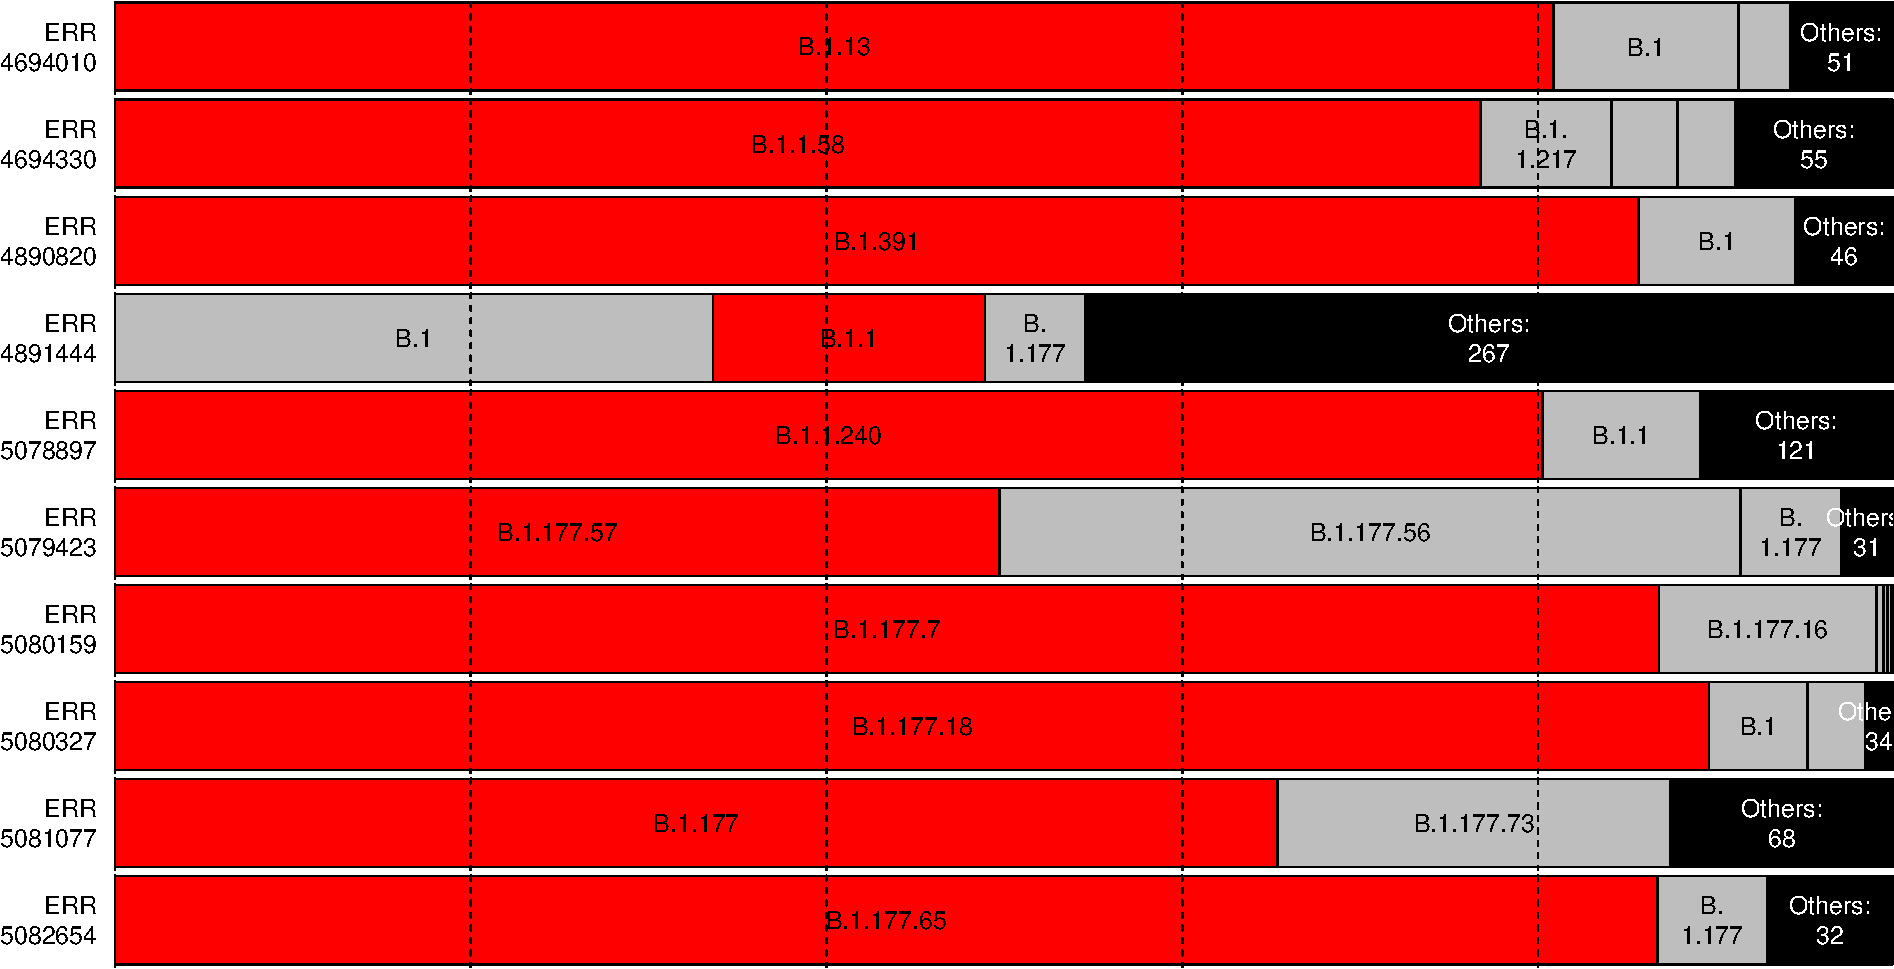
\includegraphics{pangolin_results_report_files/figure-latex/pareto-1.pdf}

\end{document}
